\documentclass[12pt]{article}
\usepackage{amscd,amssymb,amsthm,amsxtra,exscale,latexsym,verbatim,paralist}
\usepackage{mathrsfs}
\usepackage[T1]{fontenc}
\usepackage{newtxmath,newtxtext}
\usepackage[left = 2.5cm, top = 2.5cm, bottom = 2.5cm, right = 2.5cm]{geometry}

\usepackage{hyperref}
\usepackage{tikz}

\newcommand{\XB}{\color{black}}
\newcommand{\XBB}{\color{blue}}
\newcommand{\XV}{\color{violet}}
\newcommand{\XR}{\color{red}}
\newcommand{\ds}{\displaystyle}

\pagestyle{empty} 
\setlength{\parindent}{0pt} 
\setlength{\parskip}{\baselineskip}

\theoremstyle{plain}
\newtheorem{ex}{Exercise}

\renewcommand{\proofname}{Solution}

\begin{document}

\title{\textbf{MTH385}: History of Mathematics - Homework \#3}
\date{\today}
\author{\XV\textit{\large{\href{https://github.com/casonk}{Cason Konzer}}}\XB}

\maketitle

\hrulefill

\newpage
%%%%%%%%%%%%%%%%%%%%%%%%%%%%%%%%%%%%%%%%%%%%%%%%%%%%%%%%%%%%%%%%%%%%%%%%%%%%%%%%%%%%%%%%%%%%%%%%%%%%%%%%%%%%%
%%%%%%%%%%%%%%%%%%     #1     %%%%%%%%%%%%%%%%%%%%%%%%%%%%%%%%%%%%%%%%%%%%%%%%%%%%%%%%%%%%%%%%%%%%%%%%%%%%%%%
%%%%%%%%%%%%%%%%%%%%%%%%%%%%%%%%%%%%%%%%%%%%%%%%%%%%%%%%%%%%%%%%%%%%%%%%%%%%%%%%%%%%%%%%%%%%%%%%%%%%%%%%%%%%%

\XBB\hrulefill\XB \\
\begin{ex} [2.3.3]
  By finding some parallels and similar triangles in Figure~2.5, show that the diagonal $x$ of the regular pentagon of side $1$ satisfies $x/1=1/(x-1)$.
\end{ex}
\XBB\hrulefill\XB \\

\begin{center}
  \begin{tikzpicture}[scale=9.6]
    \draw [-, dashed] (-0.5,-0.951) -- (-0.809,0) -- (0,0.588) -- (0.809,0) -- (0.5,-0.951) -- (-0.5,-0.951) -- (-0.809,0) -- (0,0.588) -- (0.809,0) -- (0.5,-0.951) -- (-0.5,-0.951) -- (0.809,0) -- (-0.809,0) -- (0.5,-0.951);
    \draw [-, blue] (0,0.588) -- (-0.809,0) -- (0.809,0) -- (0,0.588);
    \draw [-, red] (0,-0.588) -- (-0.5,-0.951) -- (0.5,-0.951) -- (0,-0.588);
    \node [above left] at (-0.405,0.294) {$1$};
    \node [above right] at (0.405,0.294) {$1$};
    \node [below] at (0,-0.951) {$1$};
    \node [above] at (0,0) {$x$};
    \node [left] at (-0.809,0) {$A$};
    \node [right] at (0.809,0) {$B$};
    \node [above] at (0,0.588) {$C$};
    \node [below left] at (-0.5,-0.951) {$A'$};
    \node [below right] at (0.5,-0.951) {$B'$};
    \node [above] at (0,-0.588) {$C'$};
  \end{tikzpicture}

  Regular pentagon
\end{center}

\begin{proof}
  \ \\

  From basic principals, the interior angle at each vertex in the regular pentagon is $ \ds \theta = \frac{(5-2)\pi}{5} = \frac{3\pi}{5} $. \\
  Notice the following \dots
  \begin{itemize}
    \item $ \ds \triangle ACB $ is isosceles.
    \item $ \ds \angle ACB = \theta = \frac{3\pi}{5} $.
    \item $ \ds \angle ABC = \angle BAC = \frac{\pi}{5} $.
    \item $ \ds \triangle AA'B' $ and $ \ds \triangle BB'A' $ are similar to $ \ds \triangle ACB $.
    \item $ \ds \angle ABC = \angle A'B'C' = \angle BAC = \angle B'A'C' = \frac{\pi}{5} $.
    \item $ \ds \angle ACB = \angle A'C'B' = \frac{3\pi}{5} $.
    \item $ \ds \triangle A'C'B' $ is isosceles.
    \item $ \ds \triangle ACB $ is similar to $ \ds \triangle A'C'B' $.
  \end{itemize}

  With this established we will now move forward \dots 

  \begin{center}
    \begin{tikzpicture}[scale=7.75]
      \draw [-, dashed] (-0.5,-0.951) -- (-0.809,0) -- (0,-0.588) -- (-0.5,-0.951);
      \draw [-, red] (0,-0.588) -- (-0.5,-0.951) -- (0.5,-0.951) -- (0,-0.588);
      \node [below] at (0,-0.951) {$1$};
      \node [above left] at (-0.809,0) {$A$};
      \node [below left] at (-0.5,-0.951) {$A'$};
      \node [below left] at (-0.655,-0.475) {$1$};
      \node [above right] at (-0.35,-0.951) {$\ds \frac{\pi}{5}$};
      \node [below right] at (0.5,-0.951) {$B'$};
      \node [above] at (0,-0.588) {$C'$};
      \node [above right] at (0.225,-0.75) {$x - 1$};
      \node [below] at (0,-0.598) {$\ds \frac{3\pi}{5}$};
      \node [left] at (-0.05,-0.588) {$\ds \frac{2\pi}{5}$};
    \end{tikzpicture}

    Truncated pentagon
  \end{center}

  The above truncated pentagon will be useful to reference when making the following realizations \dots
  \begin{itemize}
    \item $ \ds |\overline{AA'}| = 1 $ by definition.
    \item $ \ds |\overline{AB'}| = x $ by symmetry.
    \item $ \ds \angle A'C'B' + \angle A'C'A = \pi \Rightarrow \angle A'C'A = \pi - \angle A'C'B' = \pi - \frac{3\pi}{5} = \frac{2\pi}{5} $.
    \item $ \ds \angle AA'C' + \angle B'A'C' = \frac{3\pi}{5} \Rightarrow \angle AA'C' = \frac{3\pi}{5} - \angle B'A'C' = \frac{3\pi}{5} - \frac{\pi}{5} = \frac{2\pi}{5} $.
    \item $ \ds \triangle AA'C $ is isosceles.
    \item $ \ds |\overline{AC'}| = 1 $
    \item $ \ds |\overline{AB'}| = |\overline{AC'}| + |\overline{C'B'}| \Rightarrow |\overline{C'B'}| = |\overline{AB'}| - |\overline{AC'}| = x - 1 $
  \end{itemize}

  It is now clear that as $ \ds \triangle ACB $ is similar to $ \ds \triangle A'C'B' $, the ratios $ \ds \frac{|\overline{BA}|}{|\overline{BC}|} $ and $ \ds \frac{|\overline{B'A'}|}{|\overline{B'C'}|} $ are equal. \\

  Thus as $ \ds |\overline{BA}| = x $, $ \ds |\overline{BC}| = 1 $, $ \ds |\overline{B'A'}| = 1 $, and $ \ds |\overline{B'C'}| = x - 1 $ ; We can see that $ \ds \frac{x}{1} = \frac{1}{x-1} $.
\end{proof}

\newpage
%%%%%%%%%%%%%%%%%%%%%%%%%%%%%%%%%%%%%%%%%%%%%%%%%%%%%%%%%%%%%%%%%%%%%%%%%%%%%%%%%%%%%%%%%%%%%%%%%%%%%%%%%%%%%
%%%%%%%%%%%%%%%%%%     #2     %%%%%%%%%%%%%%%%%%%%%%%%%%%%%%%%%%%%%%%%%%%%%%%%%%%%%%%%%%%%%%%%%%%%%%%%%%%%%%%
%%%%%%%%%%%%%%%%%%%%%%%%%%%%%%%%%%%%%%%%%%%%%%%%%%%%%%%%%%%%%%%%%%%%%%%%%%%%%%%%%%%%%%%%%%%%%%%%%%%%%%%%%%%%%
\XBB\hrulefill\XB \\
\begin{ex} [2.3.4]
  Deduce from Exercise~2.3.3 that the diagonal of the pentagon is $(1+\sqrt{5})/2$ and hence that the regular pentagon is constructible.
\end{ex}
\XBB\hrulefill\XB \\

\begin{proof}
  \ \\

  This proof will leverage the ratio derived above and the quadratic equation \dots
  \begin{itemize}
    \item $ \ds \frac{x}{1} = \frac{1}{x-1} $.
    \item $ \ds x(x-1) = x^{2} - x = 1 \Rightarrow x^{2} - x - 1 = 0 $.
    \item $ \ds x = \frac{-(-1) \pm \sqrt{(-1)^{2} - 4(1)(-1)}}{2(1)} = \frac{1 \pm \sqrt{1 + 4}}{2} = \frac{1 \pm \sqrt{5}}{2} $.
    \item $ \ds \frac{1 - \sqrt{5}}{2} < 0 $
  \end{itemize}

  Thus we have the diagonal of the pentagon is $ \ds x = \frac{1 + \sqrt{5}}{2} $ and hence that the regular pentagon is constructible.
\end{proof}

\newpage
%%%%%%%%%%%%%%%%%%%%%%%%%%%%%%%%%%%%%%%%%%%%%%%%%%%%%%%%%%%%%%%%%%%%%%%%%%%%%%%%%%%%%%%%%%%%%%%%%%%%%%%%%%%%%
%%%%%%%%%%%%%%%%%%     #3     %%%%%%%%%%%%%%%%%%%%%%%%%%%%%%%%%%%%%%%%%%%%%%%%%%%%%%%%%%%%%%%%%%%%%%%%%%%%%%%
%%%%%%%%%%%%%%%%%%%%%%%%%%%%%%%%%%%%%%%%%%%%%%%%%%%%%%%%%%%%%%%%%%%%%%%%%%%%%%%%%%%%%%%%%%%%%%%%%%%%%%%%%%%%%
\XBB\hrulefill\XB \\
\begin{ex} [2.4.2]
  By introducing suitable coordinate axes, show that a curve with the above ``constant sum'' property indeed has an equation of the form
  \[
    \frac{x^2}{a^2}+\frac{y^2}{b^2}=1.
  \]
  (It is a good idea to start with the two square root terms, representing the distances $F_1P$ and $F_2P$, on opposite sides of the equation.) Show also that any equation of this form is obtainable by suitable choice of $F_1$, $F_2$, and $F_1P+F_2P$.
\end{ex}
\XBB\hrulefill\XB \\

\begin{center}
  \begin{tikzpicture}[scale=5.5]
    \draw [<->] (-1.5,0) -- (1.5,0);
    \draw [<->] (0,1) -- (0,-1);
    \draw[very thick] (-1,0) to [out=90,in=90] (1,0);
    \draw[very thick] (-1,0) to [out=-90,in=-90] (1,0);
    \draw[thick, blue] (-1,0) -- (0,0.585);
    \draw[thick, blue] (1,0) -- (0,0.585);
    \draw[thick, blue] (1,0) -- (0,0);
    \draw [fill, blue] (-1,0) circle [radius=0.0075];
    \draw [fill, blue] (1,0) circle [radius=0.0075];
    \draw [fill, blue] (0,0) circle [radius=0.0075];
    \draw [fill, blue] (0,0.585) circle [radius=0.0075];
    \draw [fill, red] (0,0.585) circle [radius=0.0055];
    \draw [fill, red] (-0.666,0) circle [radius=0.0055];
    \draw [fill, red] (0.666,0) circle [radius=0.0055];
    \draw [fill, red] (0,0) circle [radius=0.0055];
    \draw[very thick, red, dashed] (-0.666,0) -- (0,0);
    \draw[very thick, red, dashed] (0.666,0) -- (0,0.585);
    \draw[very thick, red, dashed] (-0.666,0) -- (0,0.585);
    \draw [fill, violet] (0.666,-0.449) circle [radius=0.00375];
    \draw[thick, violet, dotted] (0.666,0) -- (0.666,-0.449);
    \draw[thick, violet, dotted] (-0.666,0) -- (0.666,-0.449);
    \draw [fill, violet] (-0.666,0) circle [radius=0.00375];
    \draw [fill, violet] (0.666,0) circle [radius=0.00375];
    \node [right] at (0,0.275) {$b$};
    \node [above right] at (0,0.585) {$CV_{1}$};
    \node [below left] at (-1,0) {$V_{1}$};
    \node [below left] at (0,-0.585) {$CV_{2}$};
    \node [above right] at (1,0) {$V_{2}$};
    \node [below right] at (0,0) {$O$};
    \node [below right, violet] at (0.666,-0.45) {$P$};
    \node [below right] at (0,1) {$y$};
    \node [above left] at (1.5,0) {$x$};
    \node [above, red] at (-0.333,0) {$d$};
    \node [below, blue] at (0.5,0) {$a$};
    \node [below left, red] at (-0.666,0) {$F_{1}$};
    \node [below right, red] at (0.666,0) {$F_{2}$};
  \end{tikzpicture}

  Ellipse

  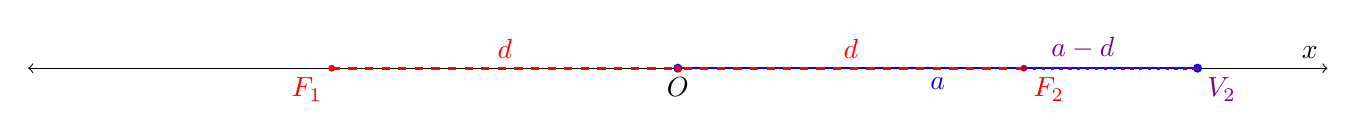
\begin{tikzpicture}[scale=6.6]
    \draw [<->] (-1.25,0) -- (1.25,0);
    \draw[thick, blue] (1,0) -- (0,0);
    \draw [fill, blue] (1,0) circle [radius=0.0075];
    \draw [fill, blue] (0,0) circle [radius=0.0075];
    \draw [fill, red] (-0.666,0) circle [radius=0.0055];
    \draw [fill, red] (0.666,0) circle [radius=0.0055];
    \draw [fill, red] (0,0) circle [radius=0.0055];
    \draw[very thick, red, dashed] (-0.666,0) -- (0,0);
    \draw[very thick, red, dashed] (0.666,0) -- (0,0);
    \draw[very thick, violet, dotted] (0.666,0) -- (1,0);
    \node [below right, violet] at (1,0) {$V_{2}$};
    \node [below] at (0,0) {$O$};
    \node [above left] at (1.25,0) {$x$};
    \node [above, red] at (-0.333,0) {$d$};
    \node [above, red] at (0.333,0) {$d$};
    \node [below, blue] at (0.5,0) {$a$};
    \node [below left, red] at (-0.666,0) {$F_{1}$};
    \node [below right, red] at (0.666,0) {$F_{2}$};
    \node [above right, violet] at (0.7,0) {$a-d$};
    \draw [fill, violet] (0.666,0) circle [radius=0.00375];
    \draw [fill, violet] (1,0) circle [radius=0.00375];
  \end{tikzpicture}

  Constant sum
\end{center}

\begin{proof}
  \ \\

  Notes: 
  \begin{itemize}
    \item Variables are taken from the Ellipse and Constant sum figures shown above.
    \item $ F_{1} $ and $ F_{2} $ are the foci of the ellipse.
    \item $ V_{1} $ and $ V_{2} $ are the verticies of the ellipse.
    \item $ CV_{1} $ and $ CV_{2} $ are the co-verticies of the ellipse.
    \item $ O $ is the origin of our cartesian axis and the center of the ellipse.
    \item $ d $ is the length from the center of the ellipse to either of the two foci.
    \item $ a $ is the length from the center of the ellipse to either of the two verticies.
    \item $ b $ is the length from the center of the ellipse to either of the two co-verticies.
  \end{itemize}

  We will first define the length $ l $ of the path $ \overline{F_{1}PF_{2}} $.
  As this path has constant sum for all points $ P $, we will solve for $ l $ from the trivial case; $ P = V_{2} $.
  \begin{itemize}
    \item $ \overline{F_{1}V_{2}F_{2}} = \overline{F_{1}V_{2}} + \overline{V_{2}F_{2}} $.
    \item $ \overline{F_{1}V_{2}} = d + a $.
    \item $ \overline{V_{2}F_{2}} = a - d $.
    \item $ \overline{F_{1}V_{2}F_{2}} = d + a + a - d = 2a = l $.
  \end{itemize}

  We now know that for any $ P $, the path $ \overline{F_{1}PF_{2}} $ will have constant length $ l = 2a $.
  Letting $ P = (x,y) $ we can leverage the distance equation to create the following equality \dots
  
  \begin{itemize}
    \item $ \ds l = 2a = \overline{F_{1}P} + \overline{F_{2}P} = \sqrt{(x - (-d))^{2} + (y)^{2}} + \sqrt{(x - d)^{2} + (y)^{2}} $.
    \item $ \ds 2a = \sqrt{(x + d)^{2} + y^{2}} + \sqrt{(x - d)^{2} + y^{2}} = \sqrt{x^{2} + 2dx + d^{2} + y^{2}} + \sqrt{x^{2} - 2dx + d^{2} + y^{2}} $.
  \end{itemize}
  
  \newpage

  Some rearrangment allows us to bring the roots to opposite sides and simplfy our equality \dots

  \begin{itemize}
    \item $ \ds 2a - \sqrt{x^{2} - 2dx + d^{2} + y^{2}} = \sqrt{x^{2} + 2dx + d^{2} + y^{2}} $.
    \item $ \ds 4a^{2} - 4a\sqrt{x^{2} - 2dx + d^{2} + y^{2}} + x^{2} - 2dx + d^{2} + y^{2} = x^{2} + 2dx + d^{2} + y^{2} $.
    \item $ \ds 4a^{2} - 4a\sqrt{x^{2} - 2dx + d^{2} + y^{2}} = 4dx  $.
    \item $ \ds a^{2} - dx = a\sqrt{x^{2} - 2dx + d^{2} + y^{2}} $.
    \item $ \ds a^{4} - 2dxa^{2} + d^{2}x^{2} = a^{2}(x^{2} - 2dx + d^{2} + y^{2}) = x^{2}a^{2} - 2dxa^{2} + d^{2}a^{2} + y^{2}a^{2} $.
    \item $ \ds a^{4} + d^{2}x^{2} = x^{2}a^{2} + d^{2}a^{2} + y^{2}a^{2} $.
    \item $ \ds d^{2}x^{2} - x^{2}a^{2} = d^{2}a^{2} + y^{2}a^{2} - a^{4} $.
    \item $ \ds x^{2}(d^{2} - a^{2}) = a^{2}(d^{2} + y^{2} - a^{2}) $.
    \item $ \ds \frac{x^{2}}{a^{2}} = \frac{d^{2} + y^{2} - a^{2}}{d^{2} - a^{2}} = \frac{y^{2}}{d^{2} - a^{2}} + \frac{d^{2} - a^{2}}{d^{2} - a^{2}} = \frac{y^{2}}{d^{2} - a^{2}} + 1 $.
    \item $ \ds \frac{x^{2}}{a^{2}} - \frac{y^{2}}{d^{2} - a^{2}} = 1 = \frac{x^{2}}{a^{2}} + \frac{y^{2}}{a^{2} - d^{2}} $.
  \end{itemize}

  At this step we now consider the trivial point $ P = CV_{1} = (0,b) $. By the equation above we find \dots
  
  \begin{itemize}
    \item $ \ds \frac{x^{2}}{a^{2}} + \frac{y^{2}}{a^{2} - d^{2}} = \frac{0^{2}}{a^{2}} + \frac{b^{2}}{a^{2} - d^{2}} = \frac{b^{2}}{a^{2} - d^{2}} = 1 $
    \item $ \ds b^{2} = a^{2} - d^{2} $
  \end{itemize}

  It is now evident that a curve with the above ``constant sum'' property indeed has an equation of the aformentioned form: $ \ds \frac{x^2}{a^2} + \frac{y^2}{b^2} = 1 $.
\end{proof}

\newpage

Another interesting property of the lines from the foci to a point $P$ on the ellipse is that they make equal angles with the tangent at $P$. It follows that a light ray from $F_1$ to $P$ is reflected through $F_2$. A simple proof of this can be based on the shortest-path property of reflection, shown in Figure~2.7 and discovered by the Greek scientist Heron around 100 \textsc{ce}.

\begin{center}
  \begin{tikzpicture}[scale=1.5]
    \draw [<->] (-5,0) -- (5,0);
    \node [above] at (-4.5,0) {$L$};
    \node [below left] at (-4,-2) {$F_1$};
    \node [below right] at (4,-4) {$F_2$};
    \draw [fill] (4,4) circle [radius=0.0275];
    \node [above right] at (4,4) {$\overline{F_2}$};
    \draw [-,dashed] (4,-4) -- (4,4);
    \draw [-, blue] (-4,-2) -- (-1.333,0) -- (4,-4);
    \draw [-,dotted, blue] (-1.333,0) -- (4,4);
    \node [above left, blue] at (-1.333,0) {$P$};
    \draw [-, red] (-4,-2) -- (1,0) -- (4,-4);
    \node [above left, red] at (1,0) {$P'$};
    \draw [-,dotted, red] (1,0) -- (4,4);
    \draw [fill] (4,0) circle [radius=0.0275];
    \draw [fill, blue] (-1.333,0) circle [radius=0.0275];
    \draw [fill, red] (1,0) circle [radius=0.0275];
  \end{tikzpicture}

  Shortest-path property
\end{center}

\vfill 

\textbf{Shortest-path property.} The path $F_1PF_2$ of reflection in the line $L$ from $F_1$ to $F_2$ is shorter than any other path $F_1P'F_2$ from $F_1$ to $L$ to $F_2$.

\newpage
%%%%%%%%%%%%%%%%%%%%%%%%%%%%%%%%%%%%%%%%%%%%%%%%%%%%%%%%%%%%%%%%%%%%%%%%%%%%%%%%%%%%%%%%%%%%%%%%%%%%%%%%%%%%%
%%%%%%%%%%%%%%%%%%     #4     %%%%%%%%%%%%%%%%%%%%%%%%%%%%%%%%%%%%%%%%%%%%%%%%%%%%%%%%%%%%%%%%%%%%%%%%%%%%%%%
%%%%%%%%%%%%%%%%%%%%%%%%%%%%%%%%%%%%%%%%%%%%%%%%%%%%%%%%%%%%%%%%%%%%%%%%%%%%%%%%%%%%%%%%%%%%%%%%%%%%%%%%%%%%%
\XBB\hrulefill\XB \\
\begin{ex} [2.4.3]
  Prove the shortest-path property, by considering the two paths $F_1PF_2$ and $F_1P'F_2$, where $\overline{F_2}$ is the reflection of the point $F_2$ in the line $L$.
\end{ex}
\XBB\hrulefill\XB \\

\begin{proof}
  \ \\

  It is straightforward to see that by symmetry we have similar triangles $ \triangle F_{1}PF_{2} $ and $ \triangle F_{1}P\overline{F_2} $, reguardless of where on the line $ L $ it may be that $ P $ lies.
  It follows directly that $ \ds | \overline{PF_{2}} | = | \overline{P\overline{F_2}} | $.

  We wish to minimze the path length $ l = | \overline{F_{1}PF_{2}} | $. 

  Utilizing the above information we can see \dots 

  \begin{itemize}
    \item $ l = | \overline{F_{1}PF_{2}} | = | \overline{F_{1}P} | + | \overline{PF_{2}} | = | \overline{F_{1}P} | + | \overline{P\overline{F_2}} | = | \overline{F_{1}P\overline{F_2}} | $. 
  \end{itemize}

  It is now evident that the choice for $ P $ we should choose to minimze the pathlength $ l = | \overline{F_{1}PF_{2}} | $ is the $ P $ that lies at the intersection of the line $ L $ and the path $ | \overline{F_{1}\overline{F_2}} | $.
  Under this circumstance $ | \overline{F_{1}P\overline{F_2}} | = | \overline{F_{1}\overline{F_2}} | = | \overline{F_{1}F_2} | $. 
  To chose any other point $ P $ would increase the path length $ l $ as it is well known that the shortest path between any two points is the line segment that connects them.

\end{proof}

\vfill

Thus to prove that the lines $F_1P$ and $F_2P$ make equal angles with the tangent, it is enough to show that $F_1PF_2$ is shorter than $F_1P'F_2$ for any other point $P'$ on the tangent at $P$.

\newpage
%%%%%%%%%%%%%%%%%%%%%%%%%%%%%%%%%%%%%%%%%%%%%%%%%%%%%%%%%%%%%%%%%%%%%%%%%%%%%%%%%%%%%%%%%%%%%%%%%%%%%%%%%%%%%
%%%%%%%%%%%%%%%%%%     #5     %%%%%%%%%%%%%%%%%%%%%%%%%%%%%%%%%%%%%%%%%%%%%%%%%%%%%%%%%%%%%%%%%%%%%%%%%%%%%%%
%%%%%%%%%%%%%%%%%%%%%%%%%%%%%%%%%%%%%%%%%%%%%%%%%%%%%%%%%%%%%%%%%%%%%%%%%%%%%%%%%%%%%%%%%%%%%%%%%%%%%%%%%%%%%
\XBB\hrulefill\XB \\
\begin{ex} [2.4.4]
  Prove this, using the fact that $F_1PF_2$ has the same length for all points $P$ on the ellipse.
\end{ex}
\XBB\hrulefill\XB \\

\begin{proof}
  \ \\

  In excersie 3 we made uses of the trivial point $ P = V_{2} $ to compute the constant sum path length $ l = 2a $. 
  It is relevant once again as we can clearly see that the path $ \overline{F_{1}PF_{2}} $ takes the shortest possible length as all points lie on the same line.
  We followed to show that this path length $ l $ is the constant for any point $ P $ on the ellipse. 
  In exercise 4 we proved that the shortest path is that which chooses $ P $ at the intersection of the line $ L $ and the line segment $ \overline{F_{1}\overline{F_2}} $. 
  We will now continue to show that the line $ L $ must be tangent to the shortest path at the turning point $ P $. 

  Consider now a revised depiction of the shortest-path property. 

  \begin{center}
    \begin{tikzpicture}[scale=1.15]
      \draw [<->] (-6.666,0) -- (6.666,0);
      \node [above] at (-6,0) {$L$};
      \node [below left] at (-4,-2) {$F_1$};
      \node [above left] at (-4,2) {$\overline{F_1}$};
      \node [above left] at (-4,0) {$F_{1}^{*}$};
      \node [below right] at (4,-4) {$F_2$};
      \node [above right] at (4,4) {$\overline{F_2}$};
      \node [above right] at (4,0) {$F_{2}^{*}$};
      \draw [-,dashed] (4,-4) -- (4,4);
      \draw [-,dashed] (-4,-2) -- (-4,2);
      \draw [-, blue] (-4,-2) -- (-1.333,0) -- (4,-4);
      \draw [-, violet] (-4,-2) -- (4,-4);
      \draw [-,dotted, blue] (-4,2) -- (-1.333,0) -- (4,4);
      \draw [-,dotted, violet] (-4,2) -- (4,4);
      \draw [fill] (4,0) circle [radius=0.0275];
      \draw [fill] (-4,0) circle [radius=0.0275];
      \draw [fill, blue] (-4,2) circle [radius=0.0275];
      \draw [fill, blue] (-4,-2) circle [radius=0.0275];
      \draw [fill, blue] (-1.333,0) circle [radius=0.0275];
      \draw [fill, blue] (4,4) circle [radius=0.0275];
      \draw [fill, blue] (4,-4) circle [radius=0.0275];
      \node [above, blue] at (-1.333,0) {$P$};
      \node [below] at (-1.333,0) {$\theta$};
      \node [below left] at (-2,0) {$\frac{\pi - \theta}{2}$};
      \node [below right] at (-0.666,0) {$\frac{\pi - \theta}{2}$};
    \end{tikzpicture}
  
    Revised shortest-path property
  \end{center}

  From the above graphic we can see three pairs of similar triangles, all of which are reflections across the line $ L $. 

  \begin{itemize}
    \item $ \ds \triangle \overline{F_{1}}PF_{1}^{*} $ is the reflection over $ L $ of $ \ds \triangle F_{1}PF_{1}^{*} $.
    \item $ \ds \triangle \overline{F_{2}}PF_{2}^{*} $ is the reflection over $ L $ of $ \ds \triangle F_{2}PF_{2}^{*} $.
    \item $ \ds \triangle \overline{F_{1}}P\overline{F_{2}} $ is the reflection over $ L $ of $ \ds \triangle F_{1}PF_{2} $.
  \end{itemize}

  Due to this symmetry we have the following equivalent angles. 

  \begin{itemize}
    \item $ \ds \angle F_{1}PF_{1}^{*} = \angle \overline{F_{1}}PF_{1}^{*} $.
    \item $ \ds \angle F_{2}PF_{2}^{*} = \angle \overline{F_{2}}PF_{2}^{*} $.
    \item $ \ds \angle F_{1}PF_{1}^{*} = \angle \overline{F_{2}}PF_{2}^{*} = \angle F_{2}PF_{2}^{*} $.
    \item $ \ds \angle F_{2}PF_{2}^{*} = \angle \overline{F_{1}}PF_{1}^{*} = \angle F_{1}PF_{1}^{*} $.
    \item $ \ds \angle F_{1}PF_{2} = \angle \overline{F_{1}}P\overline{F_{2}} $.
  \end{itemize}

  Letting $ \ds \angle F_{1}PF_{2} = \theta $, we can solve for $ \ds \angle F_{1}P\overline{F_{1}} $ and $ \ds \angle F_{1}PF_{1}^{*} $.

  \begin{itemize}
    \item $ \ds \angle F_{1}P\overline{F_{1}} = \pi - \angle F_{1}PF_{2} = \pi - \theta $.
    \item $ \ds \angle F_{1}P\overline{F_{1}} = \angle F_{1}PF_{1}^{*} + \angle \overline{F_{1}}PF_{1}^{*} = 2 \cdot \angle F_{1}PF_{1}^{*} $.
    \item $ \ds 2 \cdot \angle F_{1}PF_{1}^{*} = \pi - \theta  $.
    \item $ \ds \angle F_{1}PF_{1}^{*} = \frac{\pi - \theta}{2} $.
  \end{itemize}

  As $ \ds \angle F_{1}PF_{1}^{*} = \angle F_{2}PF_{2}^{*} = \frac{\pi - \theta}{2} $, the line $ L $ at point $ P $ is a tangent line and will be so for all values taken on by $ \theta $. 

  For good measure it is worthwile to show that indeed $ \ds \angle F_{1}PF_{1}^{*} + \angle F_{1}PF_{2} + \angle F_{2}PF_{2}^{*} = \pi $.

  \begin{itemize}
    \item  $ \ds \angle F_{1}PF_{1}^{*} + \angle F_{1}PF_{2} + \angle F_{2}PF_{2}^{*} = 2\angle F_{1}PF_{1}^{*} + \angle F_{1}PF_{2} $.
    \item  $ \ds 2\angle F_{1}PF_{1}^{*} + \angle F_{1}PF_{2} = 2 \cdot \frac{\pi - \theta}{2} + \theta = \pi - \theta + \theta = \pi $.
  \end{itemize}

  We have shown that the lines $F_1P$ and $F_2P$ make equal angles with the line $ L $, $ L $ is the tangent, 
  and as only this $ P $ lies on the line segment $ \overline{F_{1}\overline{F_{2}}} $; 
  Thus $F_1PF_2$ is shorter than $F_1P'F_2$ for any other point $P'$ on the tangent at $P$.
\end{proof}




\end{document}

